% !TeX program = lualatex
% !TeX encoding = utf8
% !TeX spellcheck = uk_UA
% !TeX root =../MexPractEng.tex

%=========================================================
\chapter{Vectors}\label{\currfilebase}
\Opensolutionfile{answer}[\currfilebase/\currfilebase-Answers]
\Writetofile{answer}{\protect\section*{\nameref*{\currfilebase}}}%
%=========================================================

\section{Adding Vectors by Components}

%=========================================================
\begin{problem}
	The position vector for an electron is $\vec r = (5.0\,m)\vec i + (3.0\,m)\vec j+ (2.0\,m)\vec k $.
	\begin{enumerate}[label = (\alph*)]
		\item Find the magnitude of $\vec r$
		\item Sketch the vector on a right-handed coordinate system.
	\end{enumerate}
\end{problem}


%=========================================================
\begin{problem}
	A positron undergoes a displacement $\Delta \vec r = (2.0\, m) \vec i - (3.0\, m) \vec j + (6.0\,m)\vec k$,
	ending with the position vector $\vec r = (3.0\, m) \vec j - (4.0\,m)\vec k$. What was the positron’s initial position vector?
\end{problem}

%=========================================================
\begin{problem}
	Two vectors are given by
	\begin{align*}
		\vec a &= 4.0\vec i - 3.0\vec j + 1.0\vec k \\
		\vec b &= -1.0\vec i + 1.0\vec j + 4.0\vec k
	\end{align*}
	In unit-vector notation, find
	 \begin{enumerate*}[label = (\alph*)]
		\item $\vec a + \vec b$, 
		\item $\vec a - \vec b$.
	\end{enumerate*}
\end{problem}


%=========================================================
\begin{problem}\label{prb:vec_roated_sc}
	In Fig.~\ref{vec_roated_sc}, a vector $\vec a$ with a magnitude of $17.0$ m is
	directed at angle $\theta = \ang{56.0}$ counterclockwise from the axis.
	What are the components 
	\begin{enumerate*}[label=(\alph*)]
		\item $a_x$
		\item and $a_y$ of the vector?
		 A second coordinate system is inclined by angle $\theta' = \ang{18.0}$ with respect to the first. What are the components 
		 \item $a_{x'}$ 
		 \item and $a_{y'}$ in this primed coordinate system?
	\end{enumerate*}
	\begin{solution}
		\begin{enumerate*}[label=(\alph*)]
			\item $9.51$~m; 
			\item $14.1$~m; 
			\item $13.4$~m;
			\item $10.5$~m.
		\end{enumerate*}
	\end{solution}
\end{problem}

%---------------------------------------------------------
\begin{figure}[h!]\centering
	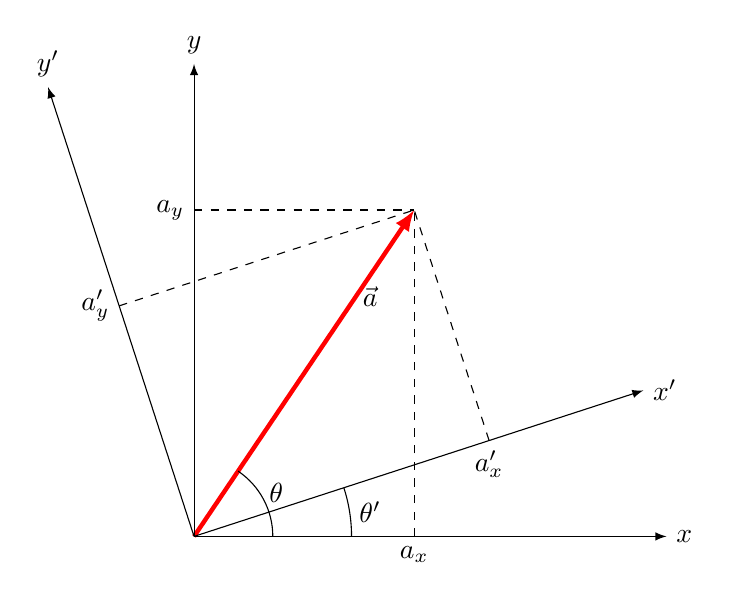
\begin{tikzpicture}
		\pgfmathsetmacro{\angone}{56}
		\pgfmathsetmacro{\angtwo}{18}
		\pgfmathsetmacro{\l}{5}
		\draw [-latex, ultra thick, red] (0,0) -- node[pos=0.8, below, text = black] {$\vec a$} (\angone:\l) coordinate (top);	
		
		\draw[-latex] (0,0) -- +(6,0) node[right] {$x$};
		\draw[-latex] (0,0) -- +(0,6) node[above] {$y$};
		\draw[dashed] (0,{\l*sin(\angone)}) node[left] {$a_y$} -- (top);	
		\draw[dashed] ({\l*cos(\angone)},0) node[below] {$a_x$} -- (top);
		\draw[] (0,0) +(0:1) arc (0:\angone:1) node[pos=0.6, right] {$\theta$};
		
		\begin{scope}[rotate=\angtwo]
			\coordinate (top2) at ({\angone - \angtwo}:\l) ;	
			\draw[-latex] (0,0) -- +(6,0) node[right] {$x'$};
			\draw[-latex] (0,0) -- +(0,6) node[above] {$y'$};
			\draw[dashed] (0,{\l*sin(\angone - \angtwo)}) node[left] {$a_y'$} -- (top2);	
			\draw[dashed] ({\l*cos(\angone - \angtwo)},0) node[below] {$a_x'$} -- (top2);
		\end{scope}
		\draw[] (0,0) +(0:2) arc (0:\angtwo:2) node[pos=0.5, right] {$\theta'$};
	\end{tikzpicture}
	\caption{Problem~\ref{prb:vec_roated_sc}}
	\label{vec_roated_sc}
\end{figure}
%---------------------------------------------------------



\section{Multiplying Vectors}

%=========================================================
\begin{problem}
	Two particles are emitted from a common source and at a particular time have displacements:
	\begin{align*}
		\vec r_1 &= 4.0\vec i + 3.0\vec j + 8.0\vec k \\
		\vec r_2 &= 2.0\vec i + 10.0\vec j + 5.0\vec k
	\end{align*}
	\begin{enumerate}[label=(\alph*)]
		\item Sketch the positions of the particles and write the expression
		for the displacement $\vec r$ of particle 2 relative to particle 1.
		\item Use the scalar product to find the magnitude of each vector.
		\item Calculate the angles between all possible pairs of the three vectors.
		\item Calculate the projection of $\vec r$ on $\vec r_1$.
		\item Calculate the vector product $\vec r_1 \times \vec r_2$. 
	\end{enumerate}
	\begin{solution}
		\begin{enumerate*}[label=(\alph*)]
			\item $\vec r = \vec r_2 - \vec r_1 = - 2.0\vec i + 7.0\vec j -3.0\vec k $
			\item $r_1 = 9.4$, $r_2 = 11.4$, $r = 7.9$.
			\item $\angle(\vec r_1, \vec r_2) = \arccos{0.7} $, $\angle(\vec r_1, \vec r) = \arccos{-0.15}$, $\angle(\vec r_2, \vec r) = \arccos{0.6}$.
			\item $-1.2$.
			\item $\vec r_1 \times \vec r_2 = -65\vec i - 4\vec j + 34 \vec k$. 
		\end{enumerate*}
	\end{solution}
\end{problem}


%=========================================================
\begin{problem}
	Find $x$ and $y$ such that the vectors $\vec b = x\vec i + 3 \vec j$ and $\vec c = 2\vec i + y \vec j$ are each perpendicular to $\vec a = 5\vec i + 6\vec j$. Now prove that $\vec b$ and $\vec c$ are parallel. Is it true in three dimensions that two vectors perpendicular to a third are necessarily parallel?
\end{problem}


%=========================================================
\begin{problem}\label{prb:vec_3_vectors}
	For the vectors in Fig.~\ref{vec_3_vectors}, with $a = 4$, $b = 3$, and $c = 5$, what are 
	\begin{enumerate*}[label=(\alph*)]
		\item the magnitude and
		\item the direction of $\vec a \times \vec b$,
		\item the magnitude and
		\item the direction of $\vec a \times \vec c$,
		\item the magnitude and
		\item the direction of $\vec b \times \vec c$.
	\end{enumerate*}
(The z axis is not shown.)
	\begin{solution}
		\begin{enumerate*}[label=(\alph*)]
			\item $12$;
			\item  $+z$;
			\item  $12$;
			\item  $-z$;
			\item  ($12$;
			\item  $+z$.
		\end{enumerate*}
	\end{solution}
\end{problem}

%---------------------------------------------------------
\begin{figure}[h!]\centering
	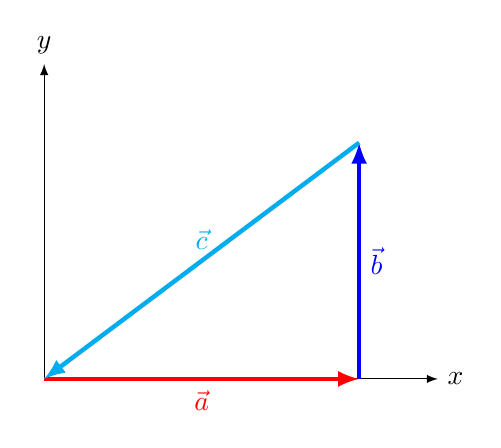
\begin{tikzpicture}
	\draw[-latex] (0,0) -- +(5,0) node[right] {$x$};
	\draw[-latex] (0,0) -- +(0,4) node[above] {$y$};
	\draw[-latex, red, ultra thick] (0,0) -- node[below] {$\vec a$} +(4,0);
	\draw[-latex, blue, ultra thick] (4,0) -- node[right] {$\vec b$} +(0,3);
	\draw[-latex, cyan, ultra thick] (4,3) -- node[above] {$\vec c$} (0,0);
	\end{tikzpicture}
	\caption{Problem~\ref{prb:vec_3_vectors}}
	\label{vec_3_vectors}
\end{figure}
%---------------------------------------------------------


\Closesolutionfile{answer}

